\documentclass[serif,mathserif,final]{beamer}
\mode<presentation>{\usetheme{Lankton}}
\usepackage[latin1]{inputenc}
\usepackage[francais]{babel}
\usepackage{amsmath,amsfonts,amssymb,pxfonts,eulervm,xspace}
\usepackage{graphicx}
\usepackage[orientation=landscape,size=custom,width=70,height=40,scale=.6,debug]{beamerposter}

%-- Header and footer information ----------------------------------
\newcommand{\footleft}{Borbot}
\newcommand{\footright}{Coupe de France de robotique 2015}
\title{Borbot}
\author{Bordelaise de robotique}
\institute{Coupe de France de robotique 2015}
%-------------------------------------------------------------------


%-- Main Document --------------------------------------------------
\begin{document}
\begin{frame}{}
  \begin{columns}[t]

    %-- Column 1 ---------------------------------------------------
    \begin{column}{0.35\linewidth}

      %-- Block 1-1
      \begin{block}{Robot principal}
        \centering
        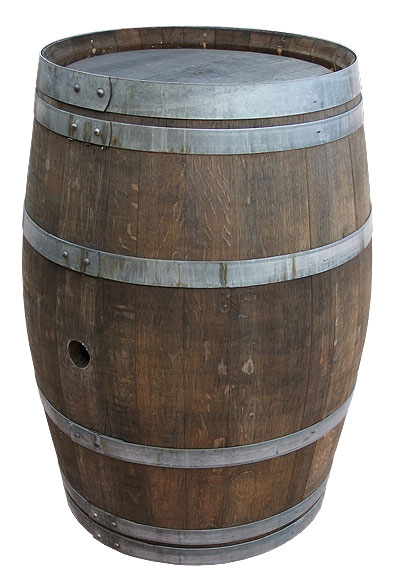
\includegraphics[height=0.19\paperwidth]{tonneau-01.jpg}
      \end{block}

      %-- Block 1-2
      \begin{block}{Actionneurs}
        Le robot principal se charge de fermer les claps et de constuire les spots.

        \vspace{1cm}
        Afin de fermer les claps le robot dispose :
        \begin{itemize}
          \item Un bras motoris� � droite
          \item un bras motoris� � gauche
        \end{itemize}

        \vspace{1cm}
        Pour la construction le robot dispose :
        \begin{itemize}
          \item Deux ascenseurs �quip�s de pinces pour faire des piles
          \item Deux taquets lat�raux afin de transferer des piles d'une pince � l'autre
        \end{itemize}
      \end{block}

      %-- Block 1-3
      \begin{block}{D�tection adversaire}
        Le robot est capable de d�tecter les adversaires gr�ce � quatres capteurs ultrason et quatres capteurs infrarouge. Le fait de coupler deux technologies permet de s'affranchir au mieux des mesures perturb�es.

        \vspace{1cm}
        Les capteurs sont r�partis entre l'avant et l'arri�re du robot (deux capteurs ultrasons et deux capteurs infrarouge de chaque cot�) de mani�re � d�tecter un adversaire en toute occasion.

        \vspace{1cm}
        Le robot est capable calculer une trajectoire d'�vitement afin de ne pas bloquer le jeu en cas de d�tection de robot adverse.
      \end{block}

    \end{column}%1

    %-- Column 2 ---------------------------------------------------
    \begin{column}{0.35\linewidth}

      %-- Block 2-1
      \begin{block}{Robot secondaire}
        \centering
        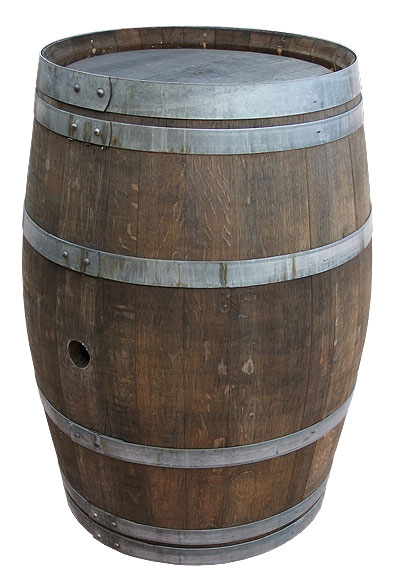
\includegraphics[height=0.19\paperwidth]{tonneau-01.jpg}
      \end{block}

      %-- Block 2-2
      \begin{block}{Actionneurs}
        Le robot secondaire se charge principalement de l'escalier.

        \vspace{1cm}
        Afin de prendre en prendre en charge l'escalier, le robot dispose : 
        \begin{itemize}
          \item Quatre pieds t�lescopique afin de monter les marches
          \item Deux pinces motoris�es afin d�poser les tapis
        \end{itemize}

        \vspace{1cm}
        Et c'est pas fini\up{\copyright~SFR} !  Le robot peux aussi d�placer des spots gr�ce � des ventouses devant et derni�re.

      \end{block}

      %-- Block 2-3
      \begin{block}{D�tection adversaire}
        Le secondaire robot est capable lui aussi de d�tecter les adversaires gr�ce � quatres capteurs ultrason et quatres capteurs infrarouge.

        \vspace{1cm}
        Les capteurs sont �galement r�partis entre l'avant et l'arri�re du robot (deux capteurs ultrasons et deux capteurs infrarouge de chaque cot�) de mani�re � d�tecter un adversaire en toute occasion.

        \vspace{1cm}
        De m�me que son compagnon, il est capable calculer une trajectoire d'�vitement afin de ne pas bloquer le jeu en cas de d�tection de robot adverse.
      \end{block}

    \end{column}%2

    %-- Column 3 ---------------------------------------------------
    \begin{column}{0.3\linewidth}

      %-- Block 3-1
      \begin{block}{Un merci au L@bx}
        le L@bx, hackerspace bordelais, nous donne la possibilit� d'avoir un endroit convivial et motivant pour cr�er nos robots.

        \vspace{1cm}
        \centering
        
\includegraphics[height=0.09\paperwidth]{logo-labx-bordeaux.pdf}
      \end{block}

      %-- Block 3-2
      \begin{block}{Merci aussi � la Fabrique Pola}
        Sans eux, rien de possible. Structure h�bergeant le L@bx, la Fabrique Pola nous a autoriser un grignoter un \emph{peu} d'espace afin d'avoir notre propre table de jeu. Indispensable pour faire un robot performant !

        \vspace{1cm}
        \centering
        
\includegraphics[height=0.09\paperwidth]{fabrique_pola.jpg}
      \end{block}

      %-- Block 3-3
      \begin{block}{N'oublions pas Plan�te Sciences}
        Sans Plan�te Sciences, point de coupe ! 

        \vspace{1cm}
        \centering
        
\includegraphics[height=0.09\paperwidth]{logo_planetesciences_national_couleur.png}
      \end{block}

    \end{column}%3

  \end{columns}
\end{frame}
\end{document}

